\def\currentRootFolder{chapter/neutrinoPhysics}
\def\currentFigureFolder{\currentRootFolder/fig}
\newacronym{standardmodel}{SM}{Standard Model of Particle Physics}
\newacronym{lep}{LEP}{Large Electron Positron Collider}
\newacronym{ssm}{SSM}{standard solar model}
\chapter{Neutrino Physics}
\label{sec:neutrinoPhysics}
This chapter is an introduction to neutrino physics. The primary aim is to give an experimentally-rooted definition of a neutrino. Therefore, in section~\ref{sec:neutrinoPhysicsHistory} selected experimental milestones are outlined that led to today's description of a neutrino within the established \gls{standardmodel}. In section~\ref{sec:neutrinoPhysicsStandardModel} follows an outline of the \gls{standardmodel} and how it relates to the neutrino. Special attention is paid to the neutrino mass: First, in section~\ref{sec:neutrinoPhysicsMassMechanisms}, an extension of the \gls{standardmodel} that allows for neutrino masses is summarized. Second, in section~\ref{sec:neutrinoPhysicsOscillations}, the phenomenon of neutrino flavor oscillations is introduced. Corresponding experiments proved that neutrinos have mass. Third, in section~\ref{sec:neutrinoPhysicsAbsoluteNuMassMeasurement}, experiments for an absolute neutrino mass measurement are presented because as such they relate particularly to the KATRIN experiment.

\section{Neutrinos until the 1960s}
\label{sec:neutrinoPhysicsHistory}
Albeit the neutrino as a hypothetical new particle was not postulated until 1930, its rich scientific history might be seen as already heralded during the preceding 35 years. 

In 1895, Becquerel reported results on experiments with phosphorescent substances, especially uranium salts, on photographic plates \cite{Becquerel:1}. These experiments mark the discovery of radioactivity and triggered manifold subsequent investigations. 

In 1899, Rutherford published a classification of radioactive decays into $\upalpha$ and $\upbeta$ types according to their penetration strength \cite{Rutherford:1}. 

In 1900, Becquerel determined the mass-charge ratio of $\upbeta$-decay particles~\cite{Becquerel:2} and identified them as the electron previously described by Thomson~\cite{Thomson:1}. 

In 1914, Chadwick measured a continuous electron energy spectrum in the $\upbeta$ decay of lead-214 and bismuth-214~\cite{Chadwick:1}. 

In 1927, Ellis and Wooster conducted a calorimetric measurement of the $\upbeta$-decay energy of radium and demonstrated that the continuity of the $\upbeta$ spectrum was intrinsic to the decay as opposed to be caused by secondary effects~\cite{Ellis:1}. 

In 1930, a $\upbeta$ decay was thought of as a two-body decay $\ce{^zA} \rightarrow \ce{^{z+1}B} + \ce{e^-}$. Assuming conservation of energy and momentum, in a two-body-decay the momenta of the daughter particles \ce{B} and \ce{e} are solely determined by their masses and the ``energy content'', as Bohr put it, of the parent particle \ce{A}. According to Bohr, there was no reason to believe that different nuclei of the same element \ce{A} should have a different energy content in a $\upbeta$ decay. Hence, the continuous nature of the $\upbeta$ spectrum could not be explained \cite{Bohr:1}. As a possible solution Pauli suggested the $\upbeta$ decay to be a three-body decay and postulated an electrically neutral particle that carries part of the decay energy~\cite{Pauli1930}. 

In 1934, Fermi developed a quantitative theory of $\upbeta$ decay that could describe the preceding experimental results~\cite{Fermi1934}. It comprises a four-fermion contact interaction respectively, a three-body-decay model. It was the first description of the so-called ``weak interaction''. Furthermore, Fermi coined the term ``neutrino'' for the particle postulated by Pauli. Fermi's theory inspired the idea to use the so-called ``inverse $\upbeta$ decay'' or ``neutrino capture'' to detect neutrinos, which in today's nomenclature is written as
\begin{equation*}
    \aeneutrino + \ce{p^+} \rightarrow \ce{n} + \ce{e^+} \fullstop
\end{equation*}

In 1956, Cowan and Reines published results of a corresponding experiment. It was conducted using the high neutrino flux of the nuclear reactor of the Savannah River Plant. The neutrinos originating in the reactor passed a tank of water and cadmium chloride triggering the above process. The emerging neutron was captured by the cadmium which emitted a photon in a \SIrange{3}{11}{MeV} range
\begin{equation*}
	n+\,^{113}\mathrm{Cd}\rightarrow \,^{114}\mathrm{Cd}+\gamma
	\fullstop
\end{equation*}
The emerging positron annihilated with an electron which produced two photons of \SI{0.5}{MeV} each. A coincidence measurement of the corresponding photons enabled discriminating signal and background events. Based on their results Cowan and Reines reported the discovery of the free neutrino~\cite{Cowan103}. 

In the same year, 1956, Lee and Yang published an article on parity conservation. Parity conservation implies that a mirrored physical process behaves the same as its non-mirrored counterpart. Here, mirroring means a change of sign of the position vector in the applied physical laws. Lee and Yang pointed out that parity conservation might be violated in weak interactions and suggested several probing methods~\cite{Lee1956}. 

In 1957 Wu et al.~conducted an experiment which employed one of the corresponding probing methods based on $\upbeta$ decay. The parity operation respectively ``the mirroring'' corresponded a change of the magnetic field orientation in the experiment. The results showed that parity is violated in weak interactions~\cite{Wu1957}. 

In 1958, Goldhaber et al.~measured the helicity $H$ of the neutrino. Helicity is defined as $ H = \unitvect{\sigma} \cdot \unitvect{p}$, where $\unitvect{\sigma}$ is the spin unit vector and $\unitvect{p}$ is the momentum unit vector (here: of the neutrino). The experiment found $H = -1$ which corresponds to maximum parity violation. In other words, only left-handed neutrinos and right-handed antineutrinos participate in weak interactions~\cite{Goldhaber1958}.

In 1962, Danby et al.~reported on a second type of neutrinos. A beam of pions generated at the Alternating Gradient Synchrotron in Brookhaven decayed according to $\uppi^{\pm} \rightarrow \upmu^{\pm} + \maybeaneutrino$. The emerging neutrinos penetrated a 13.5-meter iron shield wall and their interactions were detected in a 10-t aluminum spark chamber. The observed interactions were path-like as opposed to shower-like, which implied the production of muons as opposed to electrons. This was marked as the discovery of the muon neutrino~\cite{Danby1962}.

The attempts to uniformly describe the manifold discoveries in the field of particle physics in a combined theory converged over the course of the second half of the 20th century into what is known today as the \glsentrylong{standardmodel}.
    
\section{Neutrinos in the Standard Model of Particle Physics}
\label{sec:neutrinoPhysicsStandardModel}
This section introduces the basic concepts of the \glsentryfull{standardmodel} in a condensed manner. It aims at giving a description of relevant particle properties in section~\ref{sec:neutrinoPhysicsStandardModelParticleProperties} and relating them to neutrinos in section~\ref{sec:neutrinoPhysicsStandardModelNeutrinos}.

The \gls{standardmodel} is a gauge quantum field theory exhibiting the gauge symmetry $\text{SU}(3)\times\text{SU}(2)\times\text{U}(1)$. As such it can be formulated using the principle of least action and a Lagrangian density $\mathcal{L}$ depending on fields and their derivatives~\cite{zee2003quantum}. Albeit it can not account for all known subatomic phenomena, within its known boundaries, the \gls{standardmodel} is a well-tested and established theory, which is evident by e.\,g.~the extensive review of particle properties of the Particle Data Group~\cite{ReviewOfParticlePhysics}.

\subsection{General Particle Properties}
\label{sec:neutrinoPhysicsStandardModelParticleProperties}
The gap between fields and particles can be bridged as follows: If ``[i]n region 1 in spacetime there exists a source that sends out a `disturbance in the field', which is later absorbed by a sink in region 2 in spacetime[,] experimentalists choose to call this a particle''~\cite{zee2003quantum}. Intrinsic particle properties can be derived from the relation of their associated fields to the Lagrangian density. E.\,g., a particles's mass is encoded by the Yukawa coupling of its field to the higgs doublet through the higgs mechanism and spontaneous symmetry breaking~\cite{Higgs:1964pj}. A further intrinsic property is a particle's spin, that takes half-integer values in units of $\hbar$ for fermions or integer values for bosons. A particle's flavor is its eigenstate with respect to the weak interaction, which is described by the $\text{SU}(2)\times\text{U}(1)$ subgroup (Glashow-Weinberg-Salam model~\cite{Glashow:1961,Weinberg1967,Salam:1968}). According to Noether's theorem, each symmetry conserves an associated charge~\cite{Noether1918}. In the case of the $\text{SU}(2)\times\text{U}(1)$ symmetry, the associated charges are called isospin $\vect{T}=\transp{(T_1, T_2, T_3)}$ and hypercharge $Y$. A derivative of these charges is the electric charge $Q=T_3+\frac{1}{2}Y$~\cite{Wouter2019}. In that sense, each particle has an associated antiparticle that carries the opposite electric charge. As mentioned in the historical overview (section~\ref{sec:neutrinoPhysicsHistory}), a theory consistent with experiment must violate parity. Such theories are called chiral~\cite{zee2003quantum}. The \gls{standardmodel} is a chiral theory and thus its fermion fields can be decomposed in left- and right handed components~\cite{Wouter2019}. 

Figure~\ref{fig:standardmodel} depicts the particles of the \gls{standardmodel} along with their selected properties mass and electric charge. It also shows a further categorization among the fermions into quarks and leptons.
\FloatBarrier
\begin{figure}[t]
	\begin{center}
		\def\svgwidth{\linewidth}
		\inputpdftex{\currentFigureFolder/standardmodel}
	\end{center}
	\xcaption{The Standard Model of Particle Physics}{The Standard Model of Particle Physics.}{The diagram illustrates possible categorizations of particles within the \gls{standardmodel}. The fermions are framed with continuous and the bosons with dotted lines. Among the fermions the quark sector is marked by a thick frame and the lepton sector by a thin one. The first three columns show the fermions; and the fourth and the fifth the bosons. While the bosons in the fourth column carry a spin of 1, the higgs boson in the fifth column marked with a thicker frame carries a spin of 0. Also shown are the particle masses in natural units and their electric charge in units of the absolute electron charge. All quantities along with uncertainties can be found in the Review of Particle Physics~\cite{ReviewOfParticlePhysics}. (Illustration adapted from \cite{SeitzM2019}.)}
	\label{fig:standardmodel}
\end{figure}

\subsection{Neutrino Properties}
\label{sec:neutrinoPhysicsStandardModelNeutrinos}
With reference to the particle properties listed in the previous section~\ref{sec:neutrinoPhysicsStandardModelParticleProperties}, a neutrino can be described as follows: A neutrino carries a spin of $1/2 \hbar$. Thus, it is a fermion. It is categorized as a lepton. It has an electric charge of 0. And there are only left-handed neutrinos and right-handed antineutrinos~\cite{Wouter2019}. 

The mass of a neutrino will be discussed separately within the following chapters. 

Neutrino come in three flavors, typically denoted as $\eneutrino$, $\muneutrino$ and $\taueutrino$. Some additional remarks about the neutrino flavors can be made: First, the historical overview (section~\ref{sec:neutrinoPhysicsHistory}) mentions the discovery of the electron and muon flavor, but it was not until 2001 that the tau neutrino was discovered by the DONUT collaboration~\cite{Kodama2000}. Second, a precision measurement of the width of the \ce{Z^0}-boson resonance $\Gamma_\mathrm{Z}=\SI[separate-uncertainty=true]{2.68\pm0.15}{GeV}$ at the \gls{lep} in the 1990s yielded a number of active light neutrino flavors consistent with three. In this context, ``light'' refers to a neutrino mass smaller than half the mass $M_\mathrm{Z}=\SI{91.174\pm0.070}{GeV}$ of the \ce{Z^0}-boson~\cite{NumberOfNeutrinos}. (It should be noted that this refers to active neutrino flavors. Sterile neutrinos as an extension of the \gls{standardmodel} are not ruled out~\cite{Otten:2008zz}.)

\section{Mechanisms that Generate Neutrino Masses}
\label{sec:neutrinoPhysicsMassMechanisms}
Section~\ref{sec:neutrinoPhysicsOscillations} lists experiments which proof that neutrinos have mass. However, in the \gls{standardmodel} as described in section~\ref{sec:neutrinoPhysicsStandardModel} the neutrino masses are assumed to be zero. Nevertheless, an extension of the \gls{standardmodel} is possible. The corresponding mass terms are introduced in section~\ref{sec:neutrinoPhysicsMassMechanismsTerms}. The neutrino-mass formalism entails neutrino flavor mixing as described in section~\ref{sec:neutrinoPhysicsMassMechanismsMixing}.

\subsection{Neutrino Mass Terms}
\label{sec:neutrinoPhysicsMassMechanismsTerms}
For a theory to account for neutrino masses, its Lagrangian density must exhibit corresponding mass terms. According to~\cite{zuber2011neutrino} the formalism can be summarized: The form of a mass term is given by the Dirac equation, which is produced by applying the principle of least action to a suitable Lagrangian density $\mathcal{L}$. The mass terms have to be quadratic in the fermion fields $\psi$ and must leave the Lagrangian density hermitian. Furthermore, a field $\psi$ must have a left- and right-handed component in order for the mass terms not to vanish. Two possible term forms are named after Dirac and Majorana. Whether one or a mixture of both forms corresponds to the neutrino's reality is an open question.

\paragraph{Dirac Masses}
A Dirac mass term with mass $m_D$ split in its chiral components (Weyl spinors) $\psi_{L,R}$ has the form~\cite{zuber2011neutrino}
\begin{equation}
\mathcal{L}_D =  -m_D \bar\psi\psi = -m_D \left(\bar\psi_L\psi_R + \bar\psi_R\psi_L \right) \fullstop
\end{equation}
Applying this to neutrinos requires both a left- and a right-handed Dirac neutrino. Right-handed neutrinos have not yet been observed. If they exist, they do not interact weakly and hence are called sterile.

\paragraph{Majorana Masses}
For Majorana mass terms the CP-conjugate $\psi^C$ of a fermion spinor $\psi$ is used. It should be noted that if $\psi$ is left-handed, $\psi^C$ is right-handed and vice versa. Then, a Majorana field $\phi$ can be defined and a corresponding mass term $\mathcal{L}_M$ with a mass $m_M$ be constructed~\cite{zuber2011neutrino}:
\begin{equation}
\phi = \psi + \psi^C \qquad \mathcal{L}_M = -\frac{1}{2}m_M \bar\phi \phi \fullstop
\end{equation}
As $\phi^C=\phi$, the described Majorana particle is its own antiparticle, which due to charge conservation is only possible for neutral particles, such as a neutrino.

\subsection{Neutrino Mixing}
\label{sec:neutrinoPhysicsMassMechanismsMixing}
If neutrinos have mass, their mass eigenstates $\ket{\upnu_i}$ ($i \in \left\{1, 2, 3\right\}$) of the free Hamiltonian need not be identical to their flavor eigenstates $\ket{\upnu_\alpha}$ ($\alpha \in \left\{e,\upmu,\uptau\right\}$) of the weak interaction~\cite{zuber2011neutrino}. In case they differ, there must be a basis-change matrix. Such a matrix was introduced by Maki, Nakagawa and Sakata in order to explain the so-called neutrino oscillations (see section~\ref{sec:neutrinoPhysicsOscillations}) predicted by Pontecorvo~\cite{Pontecorvo1957, Maki1962}. Therefore, the matrix $U$ for a basis change is called Pontecorvo-Maki-Nakagawa-Sakata matrix (PMNS matrix)
\begin{equation}
\ket{\upnu_\alpha} = \sum_{i} U_{\alpha i} \ket{\upnu_i}
\fullstop
\end{equation}
As a complex unitary matrix $U$ can be expressed by six parameters. A possible choice are three angles $\theta_{12}, \theta_{23}, \theta_{13} \in [0,2\pi)$, a phase $\delta \in [0,2\pi)$ and two Majorana phases $\alpha, \beta \in [0,2\pi)$:
\begin{align}
\label{eq:PMNSmatrix}
U =  
&\begin{pmatrix} 
1 & 0 & 0 \\ 
0 & \cos\theta_{23} & \sin\theta_{23} \\ 
0 & -\sin\theta_{23} & \cos\theta_{23} 
\end{pmatrix}
\begin{pmatrix} 
\cos\theta_{13} & 0 & \sin\theta_{13}e^{-\ii\delta} \\ 
0 & 1 & 0 \\ 
-\sin\theta_{13}e^{\ii\delta} & 0 & \cos\theta_{13} 
\end{pmatrix} \\ \notag
&\begin{pmatrix} 
\cos\theta_{12} & \sin\theta_{12} & 0 \\ 
-\sin\theta_{12} & \cos\theta_{12} & 0 \\ 
0 & 0 & 1 
\end{pmatrix}
\begin{pmatrix} 
1 & 0 & 0 \\ 
0 & e^{\ii\alpha} & 0 \\ 
0 & 0 & e^{\ii\beta} 
\end{pmatrix}
\fullstop
\end{align}
These parameters are called neutrino mixing parameters. It should be noted that $\delta$ is also called ``$CP$-violating'' phase. Here, $P$ stands for parity conjugation as it was explained in section~\ref{sec:neutrinoPhysicsHistory}; and $C$ for electric charge conjugation that follows the same idea with a sign change of the electric charge instead of the position vector.  Why $\delta \neq 0$ implies $CP$-violation is shown in section~\ref{sec:neutrinoPhysicsOscillationsFormalism}.


One of the consequences of neutrino mixing, namely neutrino oscillations, will be explained in the following section \ref{sec:neutrinoPhysicsOscillations}.

\section{Neutrino Oscillations}
\label{sec:neutrinoPhysicsOscillations}
The term ``neutrino oscillations'' refers to the neutrino's change of flavor after passing a certain propagation distance. In other words, neutrinos might be detected in another flavor than the one they originated in.
Section~\ref{sec:neutrinoPhysicsOscillationsFormalism} introduces a demonstrative formalism that aims at showing the link between oscillations and the masses of neutrinos. Neutrino oscillations also depend on the neutrino mixing parameters introduced in section~\ref{sec:neutrinoPhysicsMassMechanismsMixing}. The accessibility of these mixing parameters and neutrino masses via neutrino oscillation experiments will be evaluated in section~\ref{sec:neutrinoPhysicsOscillationsMixingParams}. Neutrino oscillation experiments are manifold. As an exemplary case study the so-called ``solar neutrino problem'' is discussed in section~\ref{sec:neutrinoPhysicsOscillationsSolarExperiments}. Finally, the experimental results on neutrino oscillations will be summarized in section~\ref{sec:neutrinoPhysicsOscillationsMixingParams}. 

\subsection{Relation to Neutrino Masses}
\label{sec:neutrinoPhysicsOscillationsFormalism}
According to \cite{zuber2011neutrino} a formula demonstrating neutrino oscillations can be derived: Using the PMNS matrix $U$ from equation \eqref{eq:PMNSmatrix} the evolution of a neutrino's flavor eigenstate on a one-dimensional path starting at position $x=0$ at time $t=0$ with momentum $p_i$  and energy $E_i$ of its mass eigenstates $\ket{\upnu_i}$ is
\begin{equation}
    \ket{\upnu_\alpha(x,t)} = \sum_{i} U_{\alpha i} e^{-\ii (E_i t-p_ix)} \ket{\upnu_i} \fullstop
\end{equation}
This leads to the transition amplitudes
\begin{subequations}
    \label{eq:nuOsciTransAmp}
    \begin{equation}
    A(\alpha \rightarrow \beta)(t) 
    = \braket{\upnu_{\beta}}{\upnu_{\alpha} (x)} 
    = \sum_i U^*_{\beta i} U_{\alpha i} \euler^{-\ii (E_i t-p_ix)t}
    \end{equation}
    \begin{equation}
    A(\bar\alpha \rightarrow \bar\beta)(t) 
    = \braket{\bar{\upnu}_{\beta}}{\bar{\upnu}_{\alpha} (x)} 
    = \sum_i U_{\beta i} U^*_{\alpha i} \euler^{-\ii (E_i t-p_ix)t}
    \fullstop
    \end{equation}
\end{subequations}
It should be noted that if $U \neq U^*$, equation~\eqref{eq:nuOsciTransAmp} implies $CP$-violation. In reference to section~\ref{sec:neutrinoPhysicsMassMechanismsTerms} it holds~$U \neq U^*\Leftrightarrow\delta \neq 0$, justifying that $\delta$ is called $CP$-violating phase.

The following assumptions allow for a simple and demonstrative form of the transition probability:
\begin{itemize}
    \renewcommand{\labelitemi}{$\bullet$}
    \renewcommand{\labelitemii}{$\circ$}
    \item The neutrinos are relativistic: 
    \begin{itemize}
        \item Their momentum equals approximately their energy which is by far larger than their mass $p_i \approx E_i \gg m_i$. This also implies that the energy can be expanded in the mass-momentum-ratio $m_i/p_i$.
        \item They travel the distance $x=L=\mathrm{c}t$ at the speed of light $\mathrm{c}$.
    \end{itemize}
    \item All neutrino generations have approximately the same momentum $E \approx p \approx p_i$.
    \item The $CP$-violating phase vanishes: $\delta=0$. (This assumption is not necessary, but simplifies the expression for the transition probability. See \cite{zuber2011neutrino} for $\delta \neq 0$.)
\end{itemize}
Then, the transition probability from one flavor $\alpha$ to another $\beta$ in dependence of the neutrino masses and mixing parameters is
\begin{equation}
    \begin{split}
    P(\alpha \rightarrow \beta)(L) 
    &= \abs{\braket{\upnu_\beta}{\upnu_\alpha(L)}}^2 \\
    &= 
    \delta_{\alpha\beta}-
    4\sum_{i}\sum_{j>i} U_{\alpha i} U_{\alpha j} U_{\beta i} U_{\beta j} 
    \sin^2\left( \frac{(m_i^2-m_j^2)}{4} \frac{L}{E} \right)
    \fullstop
    \end{split}
    \label{eq:nuOsci}
\end{equation}

Equation~\eqref{eq:nuOsci} shows oscillatory behavior if two conditions are fulfilled. First, the mass eigenvalue of at least two mass eigenstates must differ. Second, the product of the corresponding PMNS matrix elements must not be zero. In other words, neutrino oscillations require at least one neutrino to have mass and to undergo flavor mixing. Furthermore, neutrino oscillation experiments are sensitive to the difference of squared masses 
\begin{equation}
    \label{eq:massSquaredDiff}
    \Delta m^2_{ij} =  \abs{m^2_i - m^2_j}
    \comma
\end{equation}
which only yields two independent observables for three masses. Thus, these experiments cannot be used to determine the absolute mass scale of neutrinos.

\subsection{Experimental Considerations}
\label{sec:neutrinoPhysicsOscillationsExpConsiderations}
According to equation \eqref{eq:nuOsci}, the ratio $L/E$ determines the sensitivity of an experiment to the oscillation parameters given by the PMNS matrix $U$ (mixing parameters) and $\Delta m^2_{ij}$ (mass ordering). $L$ can be tuned by placing the detector in a suitable distance from a Earth-based neutrino source. $E$ can either be tuned by using e.\,g.~particle accelerators as source or it varies naturally, for instance if the source exhibits an energy spectrum like e.\,g.~the Sun. 

Furthermore, two detection channels can be distinguished. If, on one hand, an experiment is only sensitive to the neutrino flavor which is emitted by the neutrino source, it can detect a weakening of the neutrino flux. This is referred to as disappearance channel. If, on the other side, an experiment is sensitive to a different neutrino flavor than the one which the neutrino source emits, this is referred to as appearance channel~\cite{zuber2011neutrino}.

There are four major classes of neutrino sources that can be used to measure the mixing parameters and the mass ordering. They are listed in table~\ref{tab:neutrinoPhysicsOscillationsExpConsiderationsParamsSources}. For each class multiple experiments exist~\cite{zuber2011neutrino}. Not all experiments will be discussed here. Instead, the following section~\ref{sec:neutrinoPhysicsOscillationsSolarExperiments} discusses the so-called ``Solar Neutrino Problem'' as an exemplary case study on solar neutrino experiments.
\FloatBarrier
\begin{table}
\begin{center}
\xcaption{Neutrino source classes for neutrino oscillation experiments}{Neutrino source classes for neutrino oscillation experiments.}{Listed are different neutrino source classes and which neutrino flavors they emit~\cite{zuber2011neutrino}. Furthermore, the oscillation parameters they are mainly sensitive to are tabulated along with an example experiment.}
    \begin{tabular}{llll}
    \toprule
         source class & flavors & sensitive to & example experiment \\
         \hline
         nuclear power plants \vphantom{{\huge A}}& $\bar{\upnu}_e$ & $\sin\theta_{13}$ & 
         Double Chooz~\cite{Abe2016}\\
         accelerators \vphantom{{\huge A}}& $\upnu_e$, $\upnu_\mu$, $\bar{\upnu}_e$, $\bar{\upnu}_\mu$ & \makecell{
         	$\sin\theta_{12}$, $\sin\theta_{23}$, \\ $\Delta m^2_{12}$, $\Delta m^2_{23}$} & 
         MiniBooNE~\cite{AGUILARAREVALO200928}\\
         atmosphere \vphantom{{\huge A}}& $\upnu_e$, $\upnu_\mu$, $\bar{\upnu}_e$, $\bar{\upnu}_\mu$ & $\sin\theta_{23}$, $\Delta m^2_{23}$ &
         Super-KamiokaNDE~\cite{Fukuda:1998mi}\\
         the Sun \vphantom{{\huge A}}& $\upnu_{e}$ & $\sin\theta_{12}$, $\Delta m^2_{21}$ & 
         SNO ~\cite{Aharmim2013}\\
    \bottomrule
    \end{tabular}
\label{tab:neutrinoPhysicsOscillationsExpConsiderationsParamsSources}
\end{center}
\end{table}

\subsection{Experimental Case Study: The Solar Neutrino Problem}
\label{sec:neutrinoPhysicsOscillationsSolarExperiments}
The term ``Solar Neutrino Problem'' refers to the mismatch of the total neutrino flux arriving on Earth predicted by the \gls{ssm} and measured by, first, the Homestake and, later, other experiments. In this section the problem is briefly described and its resolution developed.


At the end of the 1930s, Bethe, von Weizsäcker and Critchfield showed that there are two main fusion cycles in the Sun, the so-called CNO and pp cycle. The latter is the primary source of solar neutrinos \cite{Weiz1938, Bethe38, Bethe39}. Its multi-step reaction can be summarized as~\cite{zuber2011neutrino}
\begin{equation}
	\ce{4p} 
	\rightarrow 
	\ce{^4He^{2+}} +
	\ce{2e^+} +
	\ce{2\eneutrino} +
	\SI{26.73}{MeV}
	\fullstop
\end{equation}
Its initial reaction and the one with the broadest neutrino energy spectrum (from below 0.1 to $\sim\SI{11}{MeV}$ \cite{ReviewOfParticlePhysics}) are
\begin{equation}
\ce{p} + \ce{p} \rightarrow \ce{^2D} + \ce{e^+} + \upnu_e
\qquad
\ce{^8B} \rightarrow \ce{^8Be^*} + \ce{e^+} + \upnu_e \fullstop
\label{eq:ppCycle}
\end{equation}
It should be noted that only electron neutrinos are produced in the Sun. Starting from the 1970s the solar electron neutrino flux was measured; the first time by the Homestake experiment using the inverse beta decay of~\ce{^{37}Cl}. It could detect electron neutrinos with an energy threshold of~\SI{813}{keV}. The measured flux was one third of the prediction by the \gls{ssm} \cite{Cleveland1998, Bahcall2001}. This is marked as the beginning of the solar neutrino problem. The experiments GALLEX/GNO and SAGE confirmed the results, where the latter could detect electron neutrinos with an energy threshold of \SI{233}{keV}~\cite{Kirsten1998, Altmann2005, Abdurashitov2009}. The low energy threshold is of importance because the neutrinos emitted by the initial reaction of the pp cycle, equation~\eqref{eq:ppCycle}, exhibit the highest flux, but at the same time an energy spectrum that ends at approximately~\SI{400}{keV}~\cite{Bahcall1996}. 

Starting from 1999 the SNO experiment measured the neutrino flux of all flavors. It used \SI{1000}{t} of heavy water \ce{D2O} to detect electron neutrinos via charged currents as well as all flavors via neutral currents and elastic neutrino-electron scattering. In order to fully explain the flux data, the so-called Mikheyev-Smirnov-Wolfenstein effect (MSW effect) had to be respected~\cite{Wolfenstein1977, Mikheev1986}: Electron neutrinos can undergo charged current interactions with surrounding electrons in a coherent forward scattering process, which alters the flavor transition amplitude. This effect is only significant in areas of high electron densities, such as the Sun. Taking these matter-mediated oscillations into account, the measured flux of all flavors of the \ce{^8B} neutrinos, equation \eqref{eq:ppCycle}, was in accordance with the electron neutrino flux predicted by the \gls{ssm}~ \cite{Aharmim2013}. Thus, the solar neutrino problem was resolved after more than three decades.

\subsection{Summary of Experimental Results}
\label{sec:neutrinoPhysicsOscillationsMixingParams}
This section summarizes the results obtained from neutrino oscillation experiments. The neutrino oscillation parameters consist of the squared neutrino mass differences, equation~\eqref{eq:massSquaredDiff}, and the mixing parameters of the PMNS matrix, equation~\eqref{eq:PMNSmatrix}. It should be noted first, that the MSW resonance of solar neutrinos requires $m_1 < m_2$, which still allows for two possible mass orderings~\cite{zuber2011neutrino}:
\begin{enumerate}
    \item normal ordering $m_1 < m_2 < m_3$ and
    \item inverted ordering $m_3 < m_1 < m_2$.
\end{enumerate}
For these two cases a combination of recent experimental results for the neutrino oscillation parameters is given in table~\ref{tab:neutrinoPhysicsOscillationsMixingParams} and illustrated in figure~\ref{fig:neutrinoPhysicsOscillationsMixingParams}. All in all, neutrino oscillations are experimentally verified and provide unequivocal that neutrinos have mass.
\FloatBarrier
\begin{figure}[t]
	\inputpdftex[0.6\linewidth]{\currentFigureFolder/mass-hierarchy}
	\xcaption{Neutrino mixing parameters and mass ordering}{Neutrino mixing parameters and mass ordering.}{The chart shows how the mass eigenstates $\upnu_i$ are composed of the flavor eigenstates $\upnu_\alpha$ in the normal and inverted mass ordering. The composition depends on the phase $\delta$. The mixing is shown for the two extreme cases $\delta = \SI{0}{\degree}$ (baseline) and $\delta = \SI{180}{\degree}$ (topline). (Adapted from \cite{SeitzM2019}. Numerical values can be found in \cite{Esteban2019}.)}
	\label{fig:neutrinoPhysicsOscillationsMixingParams}
\end{figure}

\begin{table}
\begin{center}
	\xcaption{Overview of neutrino oscillation parameters}{Overview of neutrino oscillation parameters.}{The table lists the observables and the their best fit values along with the $1\sigma$-uncertainty range for normal and inverted ordering. (From \cite{Esteban2019}.)}
	\begin{tabular}{lll}
		\toprule
		observable & normal ordering & inverted ordering \\
		\hline
		$\sin\theta_{13}$ \vphantom{{\huge A}}&
		$0.310\substack{+0.013 \\ -0.012}$  &
		$0.310\substack{+0.013 \\ -0.012}$  \\
		$\sin\theta_{23}$ \vphantom{{\huge A}}&
		$0.580\substack{+0.017 \\ -0.021}$  &
		$0.584\substack{+0.016 \\ -0.020}$  \\  
		$\sin\theta_{13}$ \vphantom{{\huge A}}&
		$0.02241\substack{+0.00065 \\ -0.00065}$  &
		$0.02264\substack{+0.00066 \\ -0.00066}$  \\  
		$\delta / \SI{}{\degree}$ \vphantom{{\huge A}}&
		$215\substack{+40 \\ -29}$  &
		$248\substack{+27 \\ -29}$  \\
		$\frac{\Delta m^2_{21}}{\SI{e-5}{eV^2} \vphantom{\sum_1^1}}$ \vphantom{{\huge A}}&
		$7.39\substack{+0.21 \\ -0.20}$ &
		$7.39\substack{+0.21 \\ -0.20}$ \\
		$\frac{\Delta m^2_{31}}{\SI{e-3}{eV^2} \vphantom{\sum_1^1}}$ \vphantom{{\huge A}}&
		$+2.525\substack{+0.033 \\ -0.032}$&
		\\  
		$\frac{\Delta m^2_{32}}{\SI{e-3}{eV^2} \vphantom{\sum_1^1}}$ \vphantom{{\huge A}}&
		&
		$-2.512\substack{+0.034 \\ -0.032}$ \\    
		\bottomrule
	\end{tabular}
	\label{tab:neutrinoPhysicsOscillationsMixingParams}
\end{center}
\end{table}

\section{Absolute Neutrino Mass Measurements}
\label{sec:neutrinoPhysicsAbsoluteNuMassMeasurement}
The absolute masses of neutrinos remain unknown and, as shown in section~\ref{sec:neutrinoPhysicsOscillationsFormalism}, neutrino oscillations are only sensitive to squared mass differences. This section presents methods to probe the absolute neutrino mass. The corresponding measurements fall into one of three categories \cite{Otten:2008zz}:
\begin{itemize}
    \renewcommand{\labelitemi}{$\bullet$}
    \item observational cosmology (section~\ref{sec:neutrinoPhysicsAbsoluteNuMassMeasurementCosmo}),
    \item search for neutrinoless double $\upbeta$ decay (section~\ref{sec:neutrinoPhysicsAbsoluteNuMassMeasurementDoubleBeta}) or
    \item kinematic measurements of weak decays such as $\upbeta$ decay and electron capture (section~\ref{sec:neutrinoPhysicsAbsoluteNuMassMeasurementKinematics}).
\end{itemize}

\subsection{Observational Cosmology}
\label{sec:neutrinoPhysicsAbsoluteNuMassMeasurementCosmo}
In the early Universe, neutral particles such as light neutrinos could escape from areas of high mass density to areas of low mass density. As they carry away mass, the larger the neutrino mass, the stronger is the suppression of density fluctuations on small scales. In a mathematical formulation the power spectrum of the density contrast is examined and a higher neutrino mass would lead to a stronger suppression of small scale structures. Corresponding data are obtained, for example, by the Sloan Digital Sky Survey (SDSS). This survey records the sky's optical and infrared spectrum via telescope in order to map the large scale distribution of galaxies and galaxy clusters~\cite{Doroshkevich2004}. Furthermore, the temperature anisotropies in the cosmic microwave background (CMB) encode information on the Universe's structure. The latest and most precise data are recorded by the Planck satellite \cite{Aghanim:2018}. Under the assumption that all mass states contribute with the same number density cosmological observations are to first order only sensitive to the sum of all neutrino masses $\sum_{i} m_i$. A combination of the above data sets yields \cite{Yeche:2017upn}
\begin{equation*}
    \sum_i m_i < \SI{0.14}{eV} \quad (\SI{95}{\percent} \text{ C.L.}) \fullstop
\end{equation*}
\FloatBarrier

\subsection[Search for Neutrinoless Double-\texorpdfstring{$\upbeta$}{beta} Decay]{Search for Neutrinoless Double-\texorpdfstring{$\boldsymbol{\upbeta}$}{beta} Decay}
\label{sec:neutrinoPhysicsAbsoluteNuMassMeasurementDoubleBeta}
Double-$\upbeta$ decay ($2\upnu\upbeta\upbeta$) is described as a nucleus of element $\mathrm{X}(Z,A)$ with $Z$ protons and $A-Z$ neutrons that decays to a daughter isotope $\mathrm{Y}(Z+2,A)$ via two simultaneous $\upbeta$ decays 
\begin{equation}
    \mathrm{X}(Z,A) \rightarrow \mathrm{Y}(Z+2,A) + 2\mathrm{e}^- + 2\bar{\upnu}_\mathrm{e} \fullstop
\end{equation}
If the neutrino is its own antiparticle, respectively of Majorana type, the neutrino emitted in the first decay can be absorbed in the second decay resulting in a neutrinoless double decay ($0\upnu\upbeta\upbeta$). This would require the neutrino to have mass. Such a decay would manifest itself in a peak in the $\upbeta$ spectrum two neutrino masses above the endpoint of the continuum~\cite{zuber2011neutrino}. It should be noted that this would violate lepton number conservation. The half-life of such a decay encodes the Majorana mass of the electron neutrino as a coherent sum of all neutrino masses using the PMNS matrix $U$ from equation~\eqref{eq:PMNSmatrix}
\begin{equation}
    \label{eq:majoranaMass}
    m_{\upbeta\upbeta}^2 = \abs{\sum_i U_{ei}^2 m_i}^2 \fullstop
\end{equation}
As $U$ contains two unknown Majorana phases partial cancellation might occur. Hence, it is difficult to compare $m_{\upbeta\upbeta}$ to masses obtained by other methods. The two most stringent upper limits on $m_{\upbeta\upbeta}$ are listed in table~\ref{tab:neutrinoPhysicsAbsoluteNuMassMeasurementDoubleBetaResults}.

\begin{table}
	\xcaption{Constrains on the neutrino mass by double-$\upbeta$ decay experiments}{Constrains on the neutrino mass by double-$\boldsymbol{\upbeta}$ decay experiments.}{Listed are the two most stringent limits on $m_{\upbeta\upbeta}$, equation~\ref{eq:majoranaMass}, given as ranges.}
\begin{center}
	\begin{tabular}{llr}
		\toprule
		experiment & isotope & upper limit (\SI{90}{\percent} C.L.) on $m_{\upbeta\upbeta}$ (eV)\\
		\hline
		GERDA \cite{Agostini2018} & 
		\ce{^{76}Ge} \vphantom{\huge A} & 0.12–0.26 \\
		KamLAND-Zen \cite{Gando2016} & \ce{^{136}Xe} & 0.05–0.16 \\
		\bottomrule
	\end{tabular}
	\label{tab:neutrinoPhysicsAbsoluteNuMassMeasurementDoubleBetaResults}
\end{center}
\end{table}

\begin{figure}[t]
	\centering
	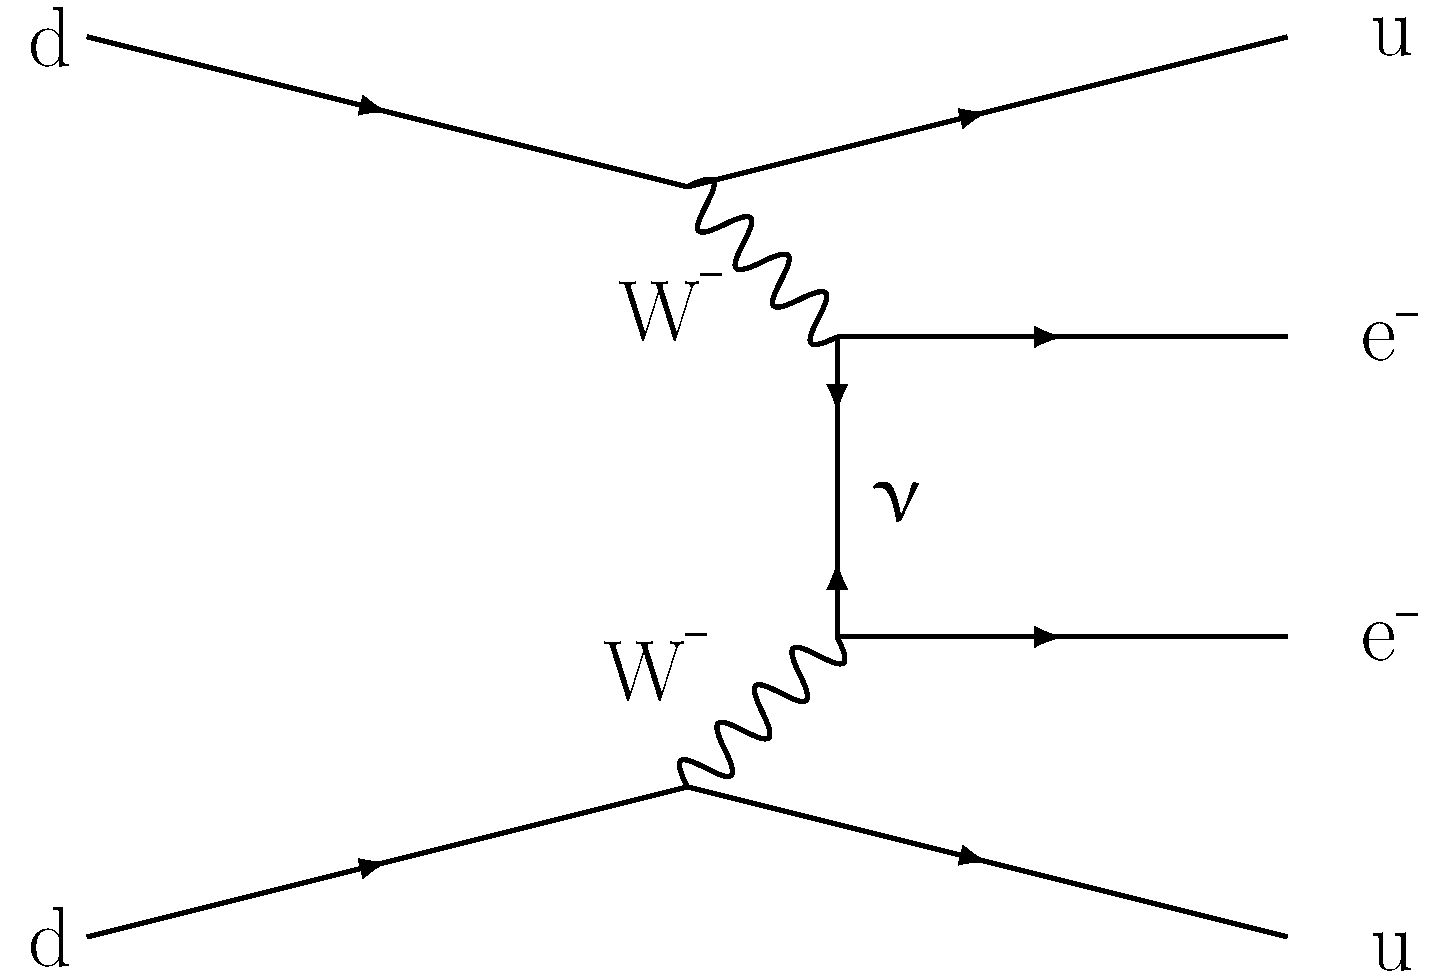
\includegraphics[width=0.4\textwidth]{\currentFigureFolder/double-beta-decay/feynman-double-beta-decay.pdf}
	\xcaption{Feynman graph of neutrinoless double-beta decay}{Feynman graph of neutrinoless double-$\boldsymbol{\upbeta}$ decay.}{The graph depicts the simultaneous transformation of two neutrons into two protons where the down quarks transform into up quarks, whilst two electrons and two neutrinos are produced. The two emitted neutrinos annihilate in a Majorana transition.}
	\label{fig:neutrinoPhysicsAbsoluteNuMassMeasurementDoubleBeta}
\end{figure}

\subsection{Kinematic Measurements of Weak Decays}
\label{sec:neutrinoPhysicsAbsoluteNuMassMeasurementKinematics}
Several laboratory experiments as well as the
supernova event 1987A have provided upper limits of absolute neutrino masses from the analysis of kinematics of weak interactions involving neutrinos or neutrino time-of-flight considerations. Such experiments can not resolve the mass splitting between the squared mass eigenvalues. Therefore, the corresponding observable is a weighted sum of the $N$ neutrino eigenmasses where the weights are the elements of the PMNS matrix from equation~\eqref{eq:PMNSmatrix}~\cite{Otten:2008zz}
\begin{equation}
\label{eq:nuMassSquared}
    m^2_{\upnu_{\alpha}} = \sum_{i}^{N}\abs{U_{\alpha i}}^2 m_i^2 \fullstop
\end{equation}
In the scope of this thesis, the measurement of the mass of the electron antineutrino via $\upbeta^-$-decay kinematics is of special interest. Hence, this subject is examined more closely within this section. For completeness, aside from the upper limit on the mass of the electron antineutrino, table~\ref{tab:neutrinoPhysicsAbsoluteNuMassMeasurementKinLimits} also lists upper limits for other neutrino flavors obtained by kinematic measurements.
\begin{table}
	\centering
	\xcaption{Constraints on the neutrino mass by kinematic measurements}{Constraints on the neutrino mass by kinematic measurements.}{The table lists upper limits on the absolute neutrino masses for different neutrino flavors.}
	\label{tab:neutrinoPhysicsAbsoluteNuMassMeasurementKinLimits}
		\begin{tabular}{llrr}
		\toprule
		flavor & measurement basis & upper limit & reference \\
		\hline
		$\upnu_\mathrm{e}$ &
		neutrinos from Supernova 1987A &
		\makecell[r]{\SI{5.7}{eV} (\SI{95}{\percent} C.I.)} &
		\cite{Loredo2002} \\
		$\upnu_\upmu$ &
		muon decay &
		\SI{17}{keV} (\SI{90}{\percent} C.L.) &
		\cite{Assamagan1996} \\
		$\upnu_\uptau$ &
		tau decay &
		\SI{18.2}{MeV} (\SI{95}{\percent} C.L.) &
		\cite{Barate:1997zg} \\
		$\aeneutrino$ &
		tritium-$\upbeta$ decay &
		\SI{2}{eV} (\SI{95}{\percent} C.L.) &
		\makecell[r]{\cite{Kraus2005}, \cite{Aseev:2011dq}, \\ \cite{ReviewOfParticlePhysics}} \\
		\bottomrule
	\end{tabular}
\end{table}


\paragraph{Neutrino Masses from $\boldsymbol{\upbeta}$-decay Kinematics} 
In $\upbeta^-$ decay
\begin{equation}
    \ce{X}(Z,A) \rightarrow \ce{Y}(Z+1,A) + \ce{e^-} + \aeneutrino
\end{equation}
part of the released surplus energy generates the neutrino's mass. This leaves a signature in the $\upbeta$ spectrum. (Also see section \ref{sec:intSpecModelDiffSpec}.) In a neutrino mass experiment four criteria  are important for a suitable $\upbeta$ emitter~\cite{Otten:2008zz}:
\begin{itemize}
	\item The $\upbeta$ emitter should have an energy spectrum with a relatively low endpoint, because in the uncertainty on the neutrino mass enter the input uncertainties of neutrino energy and	momentum scaled up with the endpoint energy.
	\item The $\upbeta$ emitter must have a sufficiently high activity to provide statistically relevant count rates for quantities that can be handled in the laboratory.
	\item The $\upbeta$ decay should be super-allowed in order for the nuclear matrix element of the decay process to be energy independent.
	\item The $\upbeta$-emitter molecule should be as simple as possible to allow for a theoretical treatment of its decay kinematics such as the final state of the decay-daughter molecule.
\end{itemize}
Tritium is an ideal candidate with respect to these criteria~\cite{Otten:2008zz}. The corresponding measurement principle will be explained more closely in the following chapters about the KATRIN experiment. However, KATRIN has several predecessor experiments. The most recent two experiments based on tritium-$\upbeta$ decay in Mainz and Troitsk obtained a combined upper limit on the electron antineutrino mass of~\cite{Kraus2005, Aseev:2011dq, ReviewOfParticlePhysics}
\begin{equation*}
    m_{\aeneutrino} < \SI{2}{eV} \quad (\SI{95}{\percent} \text{ C.L.}) \fullstop 
\end{equation*}
It should be noted that KATRIN aims for a precision that is better by one order of magnitude.
\FloatBarrier